\documentclass{mwhittaker}
\title{Bipartisan Paxos}

\usepackage{appendix}
\usepackage{mdframed}
\usepackage{multirow}
\usepackage{pervasives}
\usepackage{subcaption}
\usepackage{tikz}
\usetikzlibrary{calc}
\usetikzlibrary{positioning}
\usetikzlibrary{shapes.misc}

\theoremstyle{definition}
\newmdtheoremenv[innertopmargin=0pt]{boxedinvariant}{Invariant}

\newcommand{\todo}[2]{\textcolor{red}{TODO(#1): #2}}
\newcommand{\deps}[1]{\text{deps}(#1)}
\newcommand{\invlabel}[1]{\label{invariant:#1}}
\newcommand{\invref}[1]{Invariant~\ref{invariant:#1}}

\begin{document}
\maketitle

\begin{abstract}
  Egalitarian Paxos~\cite{moraru2013there}, or EPaxos, is a state machine
  replication protocol like Raft~\cite{ongaro2014search} or Viewstamped
  Replication~\cite{liskov2012viewstamped}. EPaxos has a number of nice features
  that set it apart from other state machine replication protocols. For example,
  it can choose non-conflicting commands in one round trip, disjoint sets of
  conflicting commands do not affect each other, and superquorum sizes are one
  node smaller than the superquorum sizes used by other protocols.
  %
  In this paper, we describe a family of consensus algorithms that are derived
  from EPaxos. We call them Bipartisan Paxos, Unanimous Bipartisan Paxos, and
  Fast Bipartisan Paxos.
\end{abstract}

\section{Bipartisan Paxos}\seclabel{BipartisanPaxos}
In this section, we describe \defword{Bipartisan Paxos}, or \defword{BPaxos}.
BPaxos is designed to be as simple to understand as possible, even at the cost
of performance. Other variants of BPaxos that we'll see later (i.e.\ Unanimous
BPaxos and Fast BPaxos) improve on BPaxos' performance.

\paragraph{Overview}
MultiPaxos allows a set of nodes to agree on a totally ordered sequence of
state machine commands. This is illustrated in \figref{MultiPaxosCartoon}.

\tikzstyle{square}=[%
  draw,
  line width=1pt,
  minimum height=0.5in,
  minimum width=0.5in,
  text width=0.4in,
  align=center
]
\begin{figure}[h]
  \centering
  \begin{tikzpicture}
    \node[square] (a) at (0, 0) {\texttt{x=1}};
    \node[square, right=-1pt of a] (b) {\texttt{y=1}};
    \node[square, right=-1pt of b] (c) {\texttt{y+=x}};
    \node[square, right=-1pt of c] (d) {\texttt{y+=1}};
    \node[square, right=-1pt of d] (e) {\texttt{x=2\\y=2}};
    \node[square, right=-1pt of e] (f) {};
    \node[square, right=-1pt of f] (g) {};
    \node[right=0in of g] (h) {\ldots};

    \foreach \label/\i in {a/0, b/1, c/2, d/3, e/4, f/5, g/6} {%
      \node[below=0in of \label] {\i};
    }
  \end{tikzpicture}
  \caption{MultiPaxos}\figlabel{MultiPaxosCartoon}
\end{figure}

While simple, agreeing on a totally ordered sequence of state machine commands
can be overly prescriptive. If two commands conflict (e.g., \texttt{x = 1} and
\texttt{x = 2}), then they \emph{do} need to be executed by every state machine
replica in the same order. But, if two commands do \emph{not} conflict (e.g.,
\texttt{x = 1} and \texttt{y = 1}), then they do \emph{not} need to be totally
ordered.  State machine replicas can execute them in either order.

EPaxos takes advantage of this fact and attempts to order commands only if they
conflict. To do so, it ditches the totally ordered sequence and instead agrees
on a directed graph of commands such that every pair of conflicting commands
have an edge between them. An example is illustrated in \figref{EPaxosCartoon}%
\footnote{%
  In reality, the graph would be the transitive closure of the one in
  \figref{EPaxosCartoon}, but we do not draw all edges to keep things simple
}.
EPaxos then executes this graph in reverse topological order one strongly
connected component at a time, executing commands within a component in an
arbitrary but deterministic order. For example, in \figref{EPaxosCartoon}, we
could execute commands in the order $R.1, R.2, S.1, Q.2, Q.1$.

\begin{figure}[h]
  \centering
  \begin{tikzpicture}[scale=2.5]
    \node[square] (a) at (0, 1) {\texttt{x=1}};
    \node[square] (b) at (0, 0) {\texttt{y=1}};
    \node[square] (c) at (1, 1) {\texttt{y+=x}};
    \node[square] (d) at (1, 0) {\texttt{y+=1}};
    \node[square] (e) at (2, 0.5) {\texttt{x=2\\y=2}};
    \draw[ultra thick, -latex] (c) to (a);
    \draw[ultra thick, -latex] (c) to (b);
    \draw[ultra thick, -latex, bend right] (c) to (e);
    \draw[ultra thick, -latex] (d) to (b);
    \draw[ultra thick, -latex, bend right] (e) to (c);
    \draw[ultra thick, -latex] (e) to (d);

    \foreach \label/\i in {a/$R.1$, b/$R.2$, c/$Q.1$, d/$S.1$, e/$Q.2$} {%
      \node[above=0in of \label] {\i};
    }
  \end{tikzpicture}
  \caption{EPaxos}\figlabel{EPaxosCartoon}
\end{figure}

Every vertex in the graph has a unique name like $Q.1$ or $R.1$. EPaxos calls
these \defword{instances}. We can view a named vertex, the command inside the
vertex, and the vertex's outbound edges as a little gadget. For example,
\figref{EPaxosGadgets} shows gadgets for instances $R.2$, $Q.1$, and $Q.2$.
%
More formally, we can think of these gadgets as tuples like $(Q.1,
\texttt{y+=x}, \set{R.1, R.2, Q.2})$ where $Q.1$ is the instance, \texttt{y+=x}
is the command in the instance, and the set $\set{R.1, R.2, Q.2}$ is the set of
\defword{dependencies} of $Q.1$ (or of \texttt{y+=x} if $Q.1$ is clear from
context).

\begin{figure}[h]
  \centering

  \begin{subfigure}[b]{0.19\textwidth}
    \begin{tikzpicture}[scale=2.5]
      \node[square] (b) at (0, 0) {\texttt{y=1}};
      \foreach \label/\i in {b/$R.2$} {%
        \node[above=0in of \label] {\i};
      }
    \end{tikzpicture}
  \end{subfigure}
  %
  \begin{subfigure}[b]{0.49\textwidth}
    \begin{tikzpicture}[scale=2.5]
      \node[square] (a) at (0, 1) {};
      \node[square] (b) at (0, 0) {};
      \node[square] (c) at (1, 1) {\texttt{y+=x}};
      \node[square] (e) at (2, 0.5) {};
      \draw[ultra thick, -latex] (c) to (a);
      \draw[ultra thick, -latex] (c) to (b);
      \draw[ultra thick, -latex, bend right] (c) to (e);
      \foreach \label/\i in {a/$R.1$, b/$R.2$, c/$Q.1$, e/$Q.2$} {%
        \node[above=0in of \label] {\i};
      }
    \end{tikzpicture}
  \end{subfigure}
  %
  \begin{subfigure}[b]{0.29\textwidth}
    \begin{tikzpicture}[scale=2.5]
      \node[square] (c) at (1, 1) {};
      \node[square] (d) at (1, 0) {};
      \node[square] (e) at (2, 0.5) {\texttt{x=2\\y=2}};
      \draw[ultra thick, -latex, bend right] (e) to (c);
      \draw[ultra thick, -latex] (e) to (d);
      \foreach \label/\i in {c/$Q.1$, d/$S.1$, e/$Q.2$} {%
        \node[above=0in of \label] {\i};
      }
    \end{tikzpicture}
  \end{subfigure}

  \caption{EPaxos Gadgets}\figlabel{EPaxosGadgets}
\end{figure}

EPaxos nodes collectively construct the directed graph of commands by stitching
together a bunch of gadgets. More precisely, an EPaxos node $R$ proposes a
gadget for instance $R.i$ and attempts to get the gadget chosen. Once a gadget
is chosen, it is considered part of the directed graph and is eligible for
execution. EPaxos' correctness hinges on the following two key invariants
(later we'll see why these invariants ensure EPaxos' correctness).

\begin{boxedinvariant}\invlabel{GadgetsChosen}
  Once a gadget $(R.i, a, \deps{a})$ has been chosen, no other gadget can be
  chosen for instance $R.i$.
\end{boxedinvariant}

\begin{boxedinvariant}\invlabel{ConflictingGadgets}
  If two gadgets $(I_a, a, \deps{a})$ and $(I_b, b, \deps{b})$ are chosen and
  commands $a$ and $b$ conflict, then either $I_a \in \deps{b}$ or $I_b \in
  \deps{a}$ or both.
\end{boxedinvariant}

BPaxos, like EPaxos, also constructs a directed graph of commands and executes
them in reverse topological order one strongly connected component at a time.
In fact, BPaxos and EPaxos execute commands in 100\% the same way. BPaxos also
maintains the same two key invariants as EPaxos. BPaxos and EPaxos differ only
in how they construct the directed graph of commands.
%
BPaxos is illustrated in \figref{BPaxos}. A BPaxos instance has three main
components: an ordering service, a consensus service, and a set of BPaxos
nodes. The ordering service helps provide \invref{ConflictingGadgets}, the
consensus service helps provide \invref{GadgetsChosen}, and the BPaxos nodes
glue the two together. We explain each of these three components in turn.

{\section{Bipartisan Paxos}
BPaxos is a modular state machine replication protocol that is both multileader
and generalized. Throughout the paper, we make the standard assumptions that
the network is asynchronous, that state machines are deterministic, and that
machines can fail by crashing but cannot act maliciously. We also assume that
at most $f$ machines can fail for some integer-valued parameter $f$. Throughput
the paper, we omit low-level protocol details involving the re-sending of
dropped messages.

\subsection{Goodbye Logs, Hello Graphs}
MultiPaxos is \emph{not} generalized. It totally orders all commands by
sequencing them into a \emph{log}. BPaxos is generalized, so it ditches the log
and instead partially orders commands into a \emph{directed graph}, like the
ones shown in \figref{ExampleBPaxosExecution}.

BPaxos graphs are completely analogous to MultiPaxos logs. Every MultiPaxos log
entry corresponds to a \defword{vertex} in a BPaxos graph. Every MultiPaxos log
entry holds a command; so does every vertex. Every log entry is uniquely
identified by it's index (e.g., \textcolor{flatred}{$0$}); every vertex is
uniquely identified by a \defword{vertex id} (e.g.,
\textcolor{flatred}{$v_0$}). The one difference between graphs and logs are the
edges. Every BPaxos vertex $v$ has edges to some set of other vertices. These
edges are called the \defword{dependencies} of $v$. Note that we view a
vertex's dependencies as belonging to the vertex, so when we refer to a vertex,
we are also referring to its dependencies. The similarities between MultiPaxos
logs and BPaxos graphs are summarized in \tabref{MultiPaxosVsBPaxos}.

\begin{table}[ht]
  \centering
  \caption{A comparison of MultiPaxos log entries and BPaxos vertices.}
  \tablabel{MultiPaxosVsBPaxos}
  \begin{tabular}{r|l}
    \textbf{BPaxos} & \textbf{MultiPaxos} \\\hline
    graph           & log \\
    vertex          & log entry \\
    vertex id       & index \\
    command         & command \\
    dependencies    & - \\
  \end{tabular}
\end{table}

MultiPaxos grows its \emph{log} over time by repeatedly reaching consensus on
one \emph{log entry} at a time. BPaxos grows its \emph{graph} over time by
repeatedly reaching consensus on one \emph{vertex} (and its dependencies) at a
time. MultiPaxos replicas execute logs in prefix order, making sure not to
execute a command until after executing \emph{all previous commands}. BPaxos
replicas execute graphs in prefix order (i.e. reverse topological order),
making sure not to execute a command until after executing \emph{its
dependencies}.

An example of how BPaxos graphs grow over time and how a BPaxos replica
executes these graphs in shown in \figref{ExampleBPaxosExecution}. As you read
through the figure, note the similarities with
\figref{ExampleMultiPaxosExecution}.
%
First, the command $a \gets 0$ is chosen in vertex $v_0$ with no dependencies
(\figref{ExampleBPaxosExecutionA}).
%
Because the vertex has no dependencies, the replica executes $a \gets 0$
immediately (\figref{ExampleBPaxosExecutionB}).
%
Next, the command $a \gets b$ is chosen in vertex $v_2$ with dependencies on
vertices $v_0$ and $v_1$ (\figref{ExampleBPaxosExecutionC}).
%
$v_2$ depends on $v_1$, but a command has not yet been chosen in $v_1$, so the
replica does \emph{not} yet execute $a \gets b$
(\figref{ExampleBPaxosExecutionD}).
%
Finally, the command $b \gets 0$ is chosen in vertex $v_1$ with no
dependencies (\figref{ExampleBPaxosExecutionE}).
%
Because $b \gets 0$ has no dependencies, the replica executes it immediately.
Moreover, all of $v_2$'s dependencies have been executed, so the replica now
executes $a \gets b$ (\figref{ExampleBPaxosExecutionF}).

{\newlength{\vertexinnersep}
\setlength{\vertexinnersep}{2pt}
\newlength{\vertexlinewidth}
\setlength{\vertexlinewidth}{1pt}
\newlength{\vertexwidth}
\setlength{\vertexwidth}{\widthof{$a \gets 1$}+2\vertexinnersep}
\newcommand{\graphindexcolor}{flatred}
\newcommand{\cmdi}{$a \gets 0$}
\newcommand{\cmdii}{$b \gets 0$}
\newcommand{\cmdiii}{$a \gets b$}
\newcommand{\xscale}{0.8}
\newcommand{\yscale}{0.75}

\tikzstyle{vertex}=[draw,
                      inner sep=\vertexinnersep,
                      line width=\vertexlinewidth,
                      minimum height=\vertexwidth,
                      minimum width=\vertexwidth]

\tikzstyle{executed}=[fill=gray, opacity=0.2, draw opacity=1, text opacity=1]

\tikzstyle{dep}=[-latex, thick]

\tikzstyle{graphindex}=[\graphindexcolor]

\begin{figure}
  \begin{subfigure}[t]{0.45\columnwidth}
    \centering
    \begin{tikzpicture}[xscale=\xscale, yscale=\yscale]
      \node[vertex, label={[graphindex]90:$v_0$}] (0) at (0, 2) {\cmdi{}};
    \end{tikzpicture}
    \caption{%
      \cmdi{} is chosen in entry $\textcolor{\graphindexcolor}{v_0}$.
    }
    \figlabel{ExampleBPaxosExecutionA}
  \end{subfigure}\hspace{0.1\columnwidth}%
  \begin{subfigure}[t]{0.45\columnwidth}
    \centering
    \begin{tikzpicture}[xscale=\xscale, yscale=\yscale]
      \node[vertex, executed, label={[graphindex]90:$v_0$}] (0) at (0, 2)
        {\cmdi{}};
    \end{tikzpicture}
    \caption{%
      \cmdi{} is executed.
    }
    \figlabel{ExampleBPaxosExecutionB}
  \end{subfigure}

  \vspace{2pt}\textcolor{flatgray}{\rule{\columnwidth}{0.4pt}}

  \begin{subfigure}[t]{0.45\columnwidth}
    \centering
    \begin{tikzpicture}[xscale=\xscale, yscale=\yscale]
      \node[vertex, executed, label={[graphindex]90:$v_0$}] (0) at (0, 2)
        {\cmdi{}};
      \node[vertex, label={[graphindex]90:$v_2$}] (2) at (2, 1) {\cmdiii{}};
      \node[vertex, label={[graphindex]90:$v_1$}] (1) at (0, 0) {};
      \draw[dep] (2) to (0);
      \draw[dep] (2) to (1);
    \end{tikzpicture}
    \caption{%
      \cmdiii{} is chosen in entry $\textcolor{\graphindexcolor}{v_2}$.
    }
    \figlabel{ExampleBPaxosExecutionC}
  \end{subfigure}\hspace{0.1\columnwidth}%
  \begin{subfigure}[t]{0.45\columnwidth}
    \centering
    \begin{tikzpicture}[xscale=\xscale, yscale=\yscale]
      \node[vertex, executed, label={[graphindex]90:$v_0$}] (0) at (0, 2)
        {\cmdi{}};
      \node[vertex, label={[graphindex]90:$v_2$}] (2) at (2, 1) {\cmdiii{}};
      \node[vertex, label={[graphindex]90:$v_1$}] (1) at (0, 0) {};
      \draw[dep] (2) to (0);
      \draw[dep] (2) to (1);
    \end{tikzpicture}
    \caption{%
      Nothing is executed.
    }
    \figlabel{ExampleBPaxosExecutionD}
  \end{subfigure}

  \vspace{2pt}\textcolor{flatgray}{\rule{\columnwidth}{0.4pt}}

  \begin{subfigure}[t]{0.45\columnwidth}
    \centering
    \begin{tikzpicture}[xscale=\xscale, yscale=\yscale]
      \node[vertex, executed, label={[graphindex]90:$v_0$}] (0) at (0, 2)
        {\cmdi{}};
      \node[vertex, label={[graphindex]90:$v_2$}] (2) at (2, 1) {\cmdiii{}};
      \node[vertex, label={[graphindex]90:$v_1$}] (1) at (0, 0) {\cmdii{}};
      \draw[dep] (2) to (0);
      \draw[dep] (2) to (1);
    \end{tikzpicture}
    \caption{%
      \cmdii{} is chosen in entry $\textcolor{\graphindexcolor}{v_1}$.
    }
    \figlabel{ExampleBPaxosExecutionE}
  \end{subfigure}\hspace{0.1\columnwidth}%
  \begin{subfigure}[t]{0.45\columnwidth}
    \centering
    \begin{tikzpicture}[xscale=\xscale, yscale=\yscale]
      \node[vertex, executed, label={[graphindex]90:$v_0$}] (0) at (0, 2)
        {\cmdi{}};
      \node[vertex, executed, label={[graphindex]90:$v_2$}] (2) at (2, 1)
        {\cmdiii{}};
      \node[vertex, executed, label={[graphindex]90:$v_1$}] (1) at (0, 0)
        {\cmdii{}};
      \draw[dep] (2) to (0);
      \draw[dep] (2) to (1);
    \end{tikzpicture}
    \caption{%
      \cmdii{}, \cmdiii{} are executed.
    }
    \figlabel{ExampleBPaxosExecutionF}
  \end{subfigure}

  \caption{%
    An example of a BPaxos replica executing commands over time, as they are
    chosen.
  }
  \figlabel{ExampleBPaxosExecution}
\end{figure}
}

Before we discuss the mechanisms that BPaxos uses to construct these graphs,
note the following three graph properties.

\paragraph{Vertices are chosen once and for all}
BPaxos reaches consensus on every vertex, so once a vertex has been chosen, it
will never change. It's command won't change, it won't lose dependencies,
and it won't get new dependencies.

\paragraph{Cycles can happen, but aren't a problem}
We'll see in a moment that BPaxos graphs can sometimes be cyclic. These cycles
are a nuisance, but easily handled. Instead of executing graphs in reverse
topological order one \emph{command} at a time, replicas instead execute graphs
in reverse topological order one \emph{strongly connected component} at a time.
The commands within a strongly connected component are executed in an arbitrary
yet deterministic order (e.g., in vertex id order). This is illustrated in
\figref{ExampleBPaxosCycleExecution}.

{\newlength{\cyclevertexinnersep}
\setlength{\cyclevertexinnersep}{4pt}
\newlength{\cyclevertexlinewidth}
\setlength{\cyclevertexlinewidth}{1pt}
\newlength{\cyclevertexwidth}
\setlength{\cyclevertexwidth}{\widthof{$x$}+2\cyclevertexinnersep}
\newcommand{\graphindexcolor}{flatred}
\newcommand{\cmdi}{$a \gets 0$}
\newcommand{\cmdii}{$b \gets 0$}
\newcommand{\cmdiii}{$a \gets b$}
\newcommand{\xscale}{0.5}
\newcommand{\yscale}{0.5}

\tikzstyle{vertex}=[draw,
                    inner sep=\cyclevertexinnersep,
                    line width=\cyclevertexlinewidth,
                    minimum height=\cyclevertexwidth,
                    minimum width=\cyclevertexwidth]

\tikzstyle{executed}=[fill=gray, opacity=0.2, draw opacity=1, text opacity=1]

\tikzstyle{dep}=[-latex, thick]

\tikzstyle{graphindex}=[\graphindexcolor]

\begin{figure}
  \centering

  \begin{subfigure}[t]{0.3\columnwidth}
    \centering
    \begin{tikzpicture}[xscale=\xscale, yscale=\yscale]
      \node[vertex, executed, label={[graphindex]90:$v_x$}] (x) at (0, 1) {$x$};
      \node[vertex, label={[graphindex]90:$v_y$}] (y) at (2, 2) {$y$};
      \node[vertex, label={[graphindex]-90:$v_z$}] (z) at (2, 0) {};
      \draw[dep] (y) to (x);
      \draw[dep, bend left] (y) to (z);
    \end{tikzpicture}
    \caption{}
    \figlabel{ExampleBPaxosCycleExecutionA}
  \end{subfigure}\hspace{0.04\columnwidth}%
  \begin{subfigure}[t]{0.3\columnwidth}
    \centering
    \begin{tikzpicture}[xscale=\xscale, yscale=\yscale]
      \node[vertex, executed, label={[graphindex]90:$v_x$}] (x) at (0, 1) {$x$};
      \node[vertex, label={[graphindex]90:$v_y$}] (y) at (2, 2) {$y$};
      \node[vertex, label={[graphindex]-90:$v_z$}] (z) at (2, 0) {$z$};
      \draw[dep] (y) to (x);
      \draw[dep, bend left] (y) to (z);
      \draw[dep, bend left] (z) to (y);
    \end{tikzpicture}
    \caption{}
    \figlabel{ExampleBPaxosCycleExecutionB}
  \end{subfigure}\hspace{0.04\columnwidth}%
  \begin{subfigure}[t]{0.3\columnwidth}
    \centering
    \begin{tikzpicture}[xscale=\xscale, yscale=\yscale]
      \node[vertex, executed, label={[graphindex]90:$v_x$}] (x) at (0, 1) {$x$};
      \node[vertex, executed, label={[graphindex]90:$v_y$}] (y) at (2, 2) {$y$};
      \node[vertex, executed, label={[graphindex]-90:$v_z$}] (z) at (2, 0) {$z$};
      \draw[dep] (y) to (x);
      \draw[dep, bend left] (y) to (z);
      \draw[dep, bend left] (z) to (y);
    \end{tikzpicture}
    \caption{}
    \figlabel{ExampleBPaxosCycleExecutionB}
  \end{subfigure}

  \caption{%c
    An example of a BPaxos replica executing a cyclic graph.
    (a) $y$ cannot be exeucted until $v_z$ is chosen.
    (b) $v_z$ is chosen. $v_y$ and $v_z$ form a strongly connected component.
    (c) $y$ and $z$ are executed in an arbitrary yet deterministic order; $y$
        then $z$ or $z$ then $y$.%
  }
  \figlabel{ExampleBPaxosCycleExecution}
\end{figure}
}

\paragraph{Conflicting commands depend on each other}
Because BPaxos is generalized, only conflicting commands have to be ordered
with respect to each other. BPaxos ensures this by maintaining the following
invariant:
\begin{invariant}[\defword{dependency invariant}]\invlabel{KeyInvariant}
  If two conflicting commands $x$ and $y$ are chosen in vertices $v_x$ and
  $v_y$, then either $v_x$ depends on $v_y$ or $v_y$ depends on $v_x$ or both.
  That is, there is at least one edge between vertices $v_x$ and $v_y$.
\end{invariant}
Because every conflicting pair of commands has an edge between them, every
replica is guaranteed to execute the commands in the same order.
Non-conflicting commands do not need an edge between them and can be executed
in either order.

\subsection{Protocol Overview}
BPaxos is composed of five modules: a dependency service, a consensus service,
a set of leaders, a set of proposers, and a set of replicas. Here, we give an
overview on how these modules interact by walking through the example execution
shown in \figref{BPaxosOverview}. In the next couple of sections, we discuss
each module in more detail.

1. A client $c$ sends a state machine command $x$ to leader $l_0$. Note that
all of the leaders process commands in parallel and that clients can send
commands to any of them.

2. Upon receiving command $x$, $l_0$ generates a globally unique vertex id
$v_x$ for $x$. It then sends the message $\msg{v_x, x}$ to the dependency
service.

3. Upon receiving message $\msg{v_x, x}$, the dependency service computes a set
of dependencies $\deps{}_x$ for vertex $v_x$. It sends back the message
$\msg{v_x, x, \deps{}_x}$ to $l_0$.

4. $l_0$ forwards $\msg{v_x, x, \deps{}_x}$ to proposer $p_0$.

5. $p_0$ sends the message $\msg{v_x, x, \deps{}_x}$ to the consensus service,
proposing that the value $(x, \deps{}_x)$ be chosen in vertex $v_x$.

6. The consensus service implements one instance of consensus for every vertex.
Upon receiving $\msg{v_x, x, \deps{}_x}$, it chooses the value $(x, \deps{}_x)$
for vertex $v_x$ and notifies $p_0$ with the message $\msg{v_x, x, \deps{}_x}$.
Note that in this example, the consensus service chose the value proposed by
$p_0$. In general, the consensus service may choose some other value if other
proposers are concurrently proposing different values for vertex $v_x$.
However, we'll see later that this can only happen during recovery, and is
therefore not typical.

7. After $p_0$ learns that command $x$ with dependencies $\deps{}_x$ has been
chosen in vertex $v_x$, it notifies the replicas by sending the message
$\msg{v_x, x, \deps{}_x}$.

8. Every replica manages a graph of chosen commands. Upon receiving $\msg{v_x,
x, \deps{}_x}$, the replicas add the vertex $v_x$ to their graph with command
$x$ and dependencies $\deps{}_x$. As described earlier, the replicas execute
the graph in reverse topological order. Once they've executed command $x$,
yielding output $o$, one of the replicas sends back the response to the client
$c$.

{% #1: starting point for bottom middle
% #2: width
% #3: height
\newcommand{\crown}[3]{{
  \newcommand{\start}{#1}
  \newcommand{\crownwidth}{#2}
  \newcommand{\crownheight}{#3}
  \definecolor{crownfg}{HTML}{F1C40F}
  \definecolor{crownbg}{HTML}{c9ab03}
  \path[draw=crownbg!50, fill=crownbg] \start{}
          -- ++(\crownwidth/2, \crownheight/2)
          -- ++(-\crownwidth/4, \crownheight/2)
          -- ++(-\crownwidth/4, -\crownheight/2)
          -- ++(-\crownwidth/4, \crownheight/2)
          -- ++(-\crownwidth/4, -\crownheight/2)
          -- ++(\crownwidth/2, -\crownheight/2);
  \path[draw=crownfg!50, fill=crownfg] \start{}
          -- ++(\crownwidth/2, 0)
          -- ++(0, \crownheight)
          -- ++(-\crownwidth/4, -\crownheight/2)
          -- ++(-\crownwidth/4, \crownheight/2)
          -- ++(-\crownwidth/4, -\crownheight/2)
          -- ++(-\crownwidth/4, \crownheight/2)
          -- ++(0, -\crownheight)
          -- ++(\crownwidth/2, 0);
}}

\newcommand{\halffill}[2]{{
  \newcommand{\thenode}{#1}
  \newcommand{\thecolor}{#2}
  \path[fill=\thecolor]
    ($(\thenode.west)!0.25!(\thenode.south west)$)
    -- ($(\thenode.east)!0.25!(\thenode.south east)$)
    -- (\thenode.south east)
    -- (\thenode.south west)
    -- cycle;
}}


\tikzstyle{proc}=[draw, circle, thick, inner sep=2pt]
\tikzstyle{leader}=[proc, fill=\leadercolor!25]
\tikzstyle{proposer}=[proc, fill=\proposercolor!25]
\tikzstyle{replica}=[proc, fill=\replicacolor!25]
\tikzstyle{client}=[proc, fill=\clientcolor!25]
\tikzstyle{proclabel}=[inner sep=0pt]
\tikzstyle{fakeproclabel}=[inner sep=0pt, white]
\tikzstyle{comm}=[-latex, thick]
\tikzstyle{commnum}=[fill=white, inner sep=0pt]
\tikzstyle{service}=[draw, rounded corners, align=center, thick]
\tikzstyle{depservice}=[service, draw=\depservicecolor!50]
\tikzstyle{consensus}=[service, draw=\consensuscolor]
\tikzstyle{module}=[draw, thick, flatgray, rounded corners]

\begin{figure}[t]
  \centering

  \begin{tikzpicture}[yscale=0.9, xscale=0.70]
    % Nodes
    \node[client] (c) at (0, 1.5) {$c$};
    \node[leader] (l0) at (2, 3) {$l_0$};
    \node[leader] (l1) at (4, 3) {$l_1$};
    \node[proposer] (p0) at (2, 1.5) {$p_0$};
    \node[proposer] (p1) at (4, 1.5) {$p_1$};
    \node[replica] (r0) at (2, 0) {$r_0$};
    \node[replica] (r1) at (4, 0) {$r_1$};
    \node[depservice] (depservice) at (0, 5) {Dependency\\Service};
    \node[consensus] (consensus) at (4, 5) {Consensus\\Service};

    % Modules
    \draw[module, \leadercolor!25]
      ($(l0.south west) + (-0.25, -0.25)$) rectangle
      ($(l1.north east) + (0.25, 0.25)$);
      \draw[module, \proposercolor!25]
      ($(p0.south west) + (-0.25, -0.25)$) rectangle
      ($(p1.north east) + (0.25, 0.25)$);
    \draw[module, \replicacolor!25]
      ($(r0.south west) + (-0.25, -0.25)$) rectangle
      ($(r1.north east) + (0.25, 0.25)$);

    % Labels
    \draw[black!100, comm] (c) to node[commnum]{$1$} (l0);
    \draw[black!85, comm, bend left=10] (l0) to node[commnum]{$2$} (depservice);
    \draw[black!85, comm, bend left=10] (depservice) to node[commnum]{$3$} (l0);
    \draw[black!85, comm] (l0) to node[commnum]{$4$} (p0);
    \draw[black!85, comm] (p0) to node[commnum]{$5$} (consensus);
    \draw[black!80, comm, bend left=15] (consensus) to node[commnum]{$6$} (p0);
    \draw[black!80, comm] (p0) to node[commnum]{$7$} (r0);
    \draw[black!80, comm] (p0) to node[commnum]{$7$} (r1);
    \draw[black!80, comm] (r0) to node[commnum]{$8$} (c);

    % Labels
    \node[fakeproclabel, anchor=west] (leaders) at (5, 3) {$\geq f+1$ Leaders};
    \halffill{leaders}{\leadercolor!25}
    \node[proclabel, anchor=west] at (leaders.west) {$\geq f+1$ Leaders};

    \node[fakeproclabel, anchor=west] (proposers) at (5, 1.5) {$\geq f+1$ Proposers};
    \halffill{proposers}{\proposercolor!25}
    \node[proclabel, anchor=west] at (proposers.west) {$\geq f+1$ Proposers};

    \node[fakeproclabel, anchor=west] (replicas) at (5, 0) {$\geq f+1$ Replicas};
    \halffill{replicas}{\replicacolor!25}
    \node[proclabel, anchor=west] at (replicas.west) {$\geq f+1$ Replicas};

    % Legend.
    \node[align=left, anchor=east] at ($(c.west)+(-0.5, 0.5)$) {%
      \textbf{Legend} \\
      $1$: $x$ \\
      $2$: $\msg{v_x, x}$ \\
      $3$: $\msg{v_x, x, \deps{}_x}$ \\
      $4$: $\msg{v_x, x, \deps{}_x}$ \\
      $5$: $\msg{v_x, x, \deps{}_x}$ \\
      $6$: $\msg{v_x, x, \deps{}_x}$ \\
      $7$: $\msg{v_x, x, \deps{}_x}$ \\
      $8$: $o$
    };
  \end{tikzpicture}

  \caption{An overview of BPaxos execution}
  \figlabel{BPaxosOverview}
\end{figure}
}

\subsection{Dependency Service}
When the dependency service receives a message of the form $\msg{v_x, x}$, it
replies with a set of dependencies $\deps{}_x$ for $v_x$ using the message
$\msg{v_x, x, \deps{}_x}$. The dependency service maintains the following
invariant.

\begin{invariant}[\defword{dependency service invariant}]%
  \invlabel{DepServiceInvariant}
  If the dependency service produces responses $\msg{v_x, x, \deps{}_x}$ and
  $\msg{v_y, y, \deps{}_y}$ for conflicting commands $x$ and $y$, then $v_x \in
  \deps{}_y$ or $v_y \in \deps{}_x$ or both.
\end{invariant}

That is, the dependency service computes dependencies such that conflicting
commands depend on each other. Note that the dependency service invariant
(\invref{DepServiceInvariant}) is very similar to the dependency invariant
(\invref{KeyInvariant}). This is not an accident. Only dependencies computed by
the dependency service can be chosen, so the dependency service invariant
suffices to guarantee that the dependency invariant is maintained.

Concretely, we implement the dependency service with $2f+1$ dependency service
nodes. Every dependency service node maintains a single piece of state,
\textsf{commands}. \textsf{commands} is the set of all the messages that the
dependency service node has received to date. When a dependency service node
receives message $\msg{v_x, x}$ from a leader, it computes
\[
  \deps{} = \setst{y}{\msg{v_y, y} \in \textsf{commands}
                      ~\text{and $x$ and $y$ conflict}}.
\]
It then adds $\msg{v_x, x}$ to \textsf{commands} and sends $\msg{v_x, x,
\deps{}}$ to the leader. When a leader sends a message $\msg{v_x, x}$ to the
dependency service, it sends it to every dependency service node. Upon
receiving $f + 1$ responses, $\set{\msg{v_x, x, \deps{}_1}, \ldots, \msg{v_x, x,
\deps{}_{f+1}}}$, the leader computes the final dependencies as
$\bigcup_{i=1}^{f+1} \deps{}_i$, the union of the computed dependencies.

\begin{theorem}
  The dependency service maintains \invref{DepServiceInvariant}.
\end{theorem}
\begin{proof}
  Assume the dependency service produces responses $\msg{v_x, x, \deps{}_x}$ and
  $\msg{v_y, y, \deps{}_y}$ for conflicting commands $x$ and $y$. We want to
  show that $v_x \in \deps{}_y$ or $v_y \in \deps{}_x$ or both. $\deps{}_x$ is
  the union of dependencies computed by some set $Q_x$ of $f + 1$ dependency
  service nodes. Similarly, $\deps{}_y$ is the union of dependencies computed
  by some set $Q_y$ of $f + 1$ dependency service nodes. Any two sets of $f +
  1$ nodes must intersect ($f+1$ is a majority of $2f+1$). Consider a
  dependency service node $d$ in the intersection of $Q_x$ and $Q_y$. $d$
  received both $\msg{v_x, x}$ and $\msg{v_y, y}$. Without loss of generality,
  assume it received $\msg{v_y, y}$ second. Then, when $d$ received $\msg{v_y,
  y}$, $\msg{v_x, x}$ was already in its \textsf{commands}, so it must have
  included $v_x$ in its computed dependencies for $v_y$. $\deps{}_y$ is a union
  of dependencies that includes the dependencies computed by $d$. Thus, $v_x
  \in \deps{}_y$.
\end{proof}

Note that if the dependency service produces responses $\msg{v_x, x,
\deps{}_x}$ and $\msg{v_y, y, \deps{}_y}$ for conflicting commands $x$ and $y$,
it may include $v_x \in \deps{}_y$ \emph{and} $v_y \in \deps{}_x$. For example,
if dependency service node $d_1$ receives $x$ then $y$ while dependency service
node $d_2$ receives $y$ then $x$, then dependencies formed from $d_1$ and $d_2$
will have $v_x$ and $v_y$ in each other's dependencies. This is the reason why
BPaxos graphs may develop cycles.

\subsection{Leaders}
The dependency

\subsection{Proposers and Consensus Service}
mention you can use paxos with proposers being paxos proposers and this service
implemented as paxos acceptors


\subsection{Recovery}

add pseudocode (including dep service) jk
add protocol diagram

{% https://tex.stackexchange.com/a/226010
\newcommand{\LineComment}[1]{\textcolor{gray}{// #1}}

\tikzstyle{comm}=[-latex, thick]
\tikzstyle{commnum}=[fill=white, inner sep=1pt]
\tikzstyle{proc}=[thick, text width=0.45\textwidth, anchor=north]

\begin{figure*}[t]
  \centering
  \begin{tikzpicture}
    \node[draw,
          thick,
          minimum width=6.8in,
          minimum height=0.25in]
          (clients) at (4.5, 1.25) {\large \textbf{Clients}};

    \node[proc,
          draw=\leadercolor,
          label={90:\textbf{\large Leader}}] (leader) at (0, 0) {%
      \newcommand{\leaderindex}{\textsf{leader index}}
      \newcommand{\nextid}{\textsf{next id}}
      \begin{algorithmic}[1]
        \GlobalState $\leaderindex{}$ \LineComment{e.g., $l_0$ has index $0$}
        \GlobalState $\nextid{} \gets 0$
        \Upon{receiving command $x$ from client}
          \State $v_x \gets (\leaderindex{}, \nextid{})$
          \State $\nextid{} \gets \nextid + 1$
          \State send $\msg{v_x, x}$ to dependency service nodes
        \EndUpon
        \Upon{receiving dependencies from $f + 1$ dependency service nodes for vertex $v_x$}
          \State let $\deps{}_1, \ldots, \deps{}_{f+1}$ be the dependencies
          \State $\deps{}_x \gets \bigcup_i \deps{}_i$
          \State send $\msg{v_x, x, \deps{}_x}$ to a proposer
        \EndUpon
      \end{algorithmic}
    };

    \node[proc,
          draw=\depservicecolor,
          label={90:\textbf{\large Dependency Service Node}},
          anchor=north] (depservice) at (9, 0) {%
      \newcommand{\commands}{\textsf{cmds}}
      \begin{algorithmic}[1]
        \GlobalState $\commands$ \LineComment{set of messages $\msg{v_x, x}$}
        \Upon{receiving $\msg{v_x, x}$ from leader $l$}
          \State $\deps{} = \setst{v_y}{\msg{v_y, y} \in \commands \land
                                        \text{$x$, $y$ conflict}}$
          \State send $\msg{v_x, x, \deps{}}$ to $l$
        \EndUpon
      \end{algorithmic}
    };

    \node[proc,
          draw=\proposercolor,
          label={90:\textbf{\large Proposer}},
          below=of leader] (proposer) {%
      \begin{algorithmic}[1]
        \Upon{receiving $\msg{v_x, x, \deps{}_x}$ from leader}
          \State send $\msg{v_x, x, \deps{}_x}$ to consensus service
        \EndUpon

        \Upon{receiving $\msg{v_x, x, \deps{}_x}$ from consensus service}
          \State send $\msg{v_x, x, \deps{}_x}$ to replicas
        \EndUpon
      \end{algorithmic}
    };

    \node[proc,
          draw=\consensuscolor,
          label={90:\textbf{\large Consensus Service}},
          below=of depservice] (consensus) {%
      \begin{algorithmic}[1]
        \Upon{receiving $\msg{v_x, x, \deps{}_x}$ from proposer $p$}
          \State reach consensus on $(x', \deps{}_x')$ for vertex $v_x$
          \State send $\msg{v_x, x', \deps{}_x'}$ to $p$
        \EndUpon
      \end{algorithmic}
    };

    \node[proc,
          draw=\replicacolor,
          label={90:\textbf{\large Replica}},
          below=of consensus] (replica) {%
      \newcommand{\graph}{\textsf{graph}}
      \newcommand{\replicaIndex}{\textsf{replica index}}
      \newcommand{\numReplicas}{\textsf{num replicas}}
      \begin{algorithmic}[1]
        \GlobalState $\graph$ \LineComment{BPaxos graph of chosen vertices}
        \GlobalState $\numReplicas{}$ \LineComment{the number of replicas}
        \Upon{receiving $\msg{v_x, x, \deps{}_x}$ from proposer}
          \State add $\msg{v_x, x, \deps{}_x}$ to $\graph$
          \State execute every eligible vertex $v_y$
          \If{$\text{hash}(v_y)~\%~\numReplicas = \replicaIndex$}
            \State send result of executing $v_y$ back to client
          \EndIf
        \EndUpon
      \end{algorithmic}
    };

    \draw[comm]
      ($(clients.south west)!0.72!(clients.south)$)
      to node[commnum] {$1$}
      ($(leader.north)!0.5!(leader.north east)$);
    \draw[comm, black!85]
      ($(leader.north east)!0.5!(leader.east)$)
      to node[commnum] {$2$}
      (depservice);
    \draw[comm, black!85]
      (depservice.south west) to node[commnum] {$3$} (leader.east);
    \draw[comm, black!85]
      ($(leader.south)!0.5!(leader.south east)$)
      to node[commnum] {$4$}
      ($(proposer.north)!0.5!(proposer.north east)$);
    \draw[comm, black!80] (proposer.north east) to node[commnum] {$5$} (consensus.west);
    \draw[comm, black!80] (consensus) to node[commnum] {$6$} (proposer.north east);
    \draw[comm, black!80] (proposer) to node[commnum] {$7$} (replica);
    \draw[comm, black!80]
      (replica.east) to ++(0.5, 0)
                     to node[commnum]{$8$} ++(0, 8.75)
                     to (clients.east);
  \end{tikzpicture}

  \caption{BPaxos pseudocode}
  \figlabel{BPaxosPseudocode}
\end{figure*}
}
}

\paragraph{Ordering Service}
The ordering service is responsible for computing the dependencies between
conflicting state machine commands. When a BPaxos node $R$ receives a state
machine command $a$ from a client, it chooses some instance $R.i$ for $a$.
Then, $R$ sends $a$ and $R.i$ to the ordering service. When the ordering
service receives a command $a$ for instance $R.i$, it replies with a tuple
$(R.i, a, \deps{a})$ where $\deps{a} = \set{I_1, \ldots, I_n}$ is $a$'s
dependencies.
%
The ordering service maintains the following invariant.

\begin{boxedinvariant}\invlabel{OrderingService}
If two conflicting commands $a$ and $b$ in instances $I_a$ and $I_b$ yield
responses $(I_a, a, \deps{a})$ and $(I_b, b, \deps{b})$ from the ordering
service, then either $I_a \in \deps{b}$ or $I_b \in \deps{a}$ (or both). That
is, if two conflicting commands are sent to the ordering service, at least one
is guaranteed to be a dependency of the other.
\end{boxedinvariant}

Note that the ordering service makes the following assumption. At most one
command can be sent in any given instance. BPaxos satisfies this invariant
because $R$ assigns every command $a$ to a unique instance $R.i$, and no other
EPaxos node contacts the ordering service for an instance $R.i$.

Implementing a fault tolerant ordering service is straightforward. We employ
$2f + 1$ ordering service nodes $o_{1}, \ldots, o_{2f + 1}$. When a BPaxos node
$R$ sends a command $a$ in instance $R.i$ to the ordering service, it sends the
command to all $2f + 1$ of the ordering service nodes. Every ordering service
node $o_i$ maintains a set $O_i = {(I_1, c_1), (I_2, c_2), \ldots}$ of all the
commands and corresponding instances that it has received. When node $o_i$
receives a command $a$ for instance $R.i$ from a BPaxos node, it atomically
performs two actions.
\begin{enumerate}
  \item
    $o_i$ replies to $R$ with the tuple $(R.i, a, \deps{a}_i)$ where
    $\deps{a}_i$ is the set of instances $I$ for which there exists a $(I, c)
    \in O_i$ such that $a$ and $c$ conflict. This is the set of instances that
    $o_i$ has previously received that contain a command that conflict with
    $a$.

  \item
    $o_i$ adds $(R.i, a)$ to $O_i$.
\end{enumerate}

When a BPaxos node receives replies $(R.i, a, \deps{a}_{i_1}), \ldots, (R.i, a,
\deps{a}_{i_{f+1}})$ from a quorum $Q_a$ of $f + 1$ ordering service nodes, it
takes $(R.i, a, \deps{a}_{i_1} \cup \ldots \cup \deps{a}_{i_{f+1}})$ to be the
response from the ordering service. That is, it computes $\deps{a}$ by taking
the union of $\deps{a}_i$ from a majority of the ordering service nodes.

To understand why this ordering service implementation maintains
\invref{OrderingService}, consider conflicting commands $a$ and $b$ in
instances $I_a$ and $I_b$. Assume $a$'s reply $(I_a, a, \deps{a})$ was formed
from a quorum $Q_a$ and $b$'s reply $(I_b, b, \deps{b})$ was formed from a
quorum $Q_b$. Any two quorums intersect, so $Q_a \cap Q_b$ is nonempty. Let
$o_i$ be an ordering service node in this intersection. $o_i$ either received
$a$ or $b$ first. If it received $a$ first, then $(I_a, a)$ is in $O_i$ when
$o_i$ processed command $b$, so $o_i$ includes $I_a$ in $\deps{b}_i$, so $I_a$
is in $\deps{b}$.  Symmetrically, if $o_i$ received $b$ first, then it includes
$I_b$ in $\deps{a}$.

\paragraph{Consensus Service}
We assume we have some set $p_1, \ldots, p_n$ of nodes that implement Plain
Jane consensus. A BPaxos node can propose to the consensus service that some
value $v$ be chosen in some instance $I$. The consensus service replies with
the value that has been chosen in instance $I$, which may or may not be $v$
depending on if there are concurrent proposers proposing to instance $i$. The
consensus service guarantees that for every instance $I$, at most one value is
ever chosen in $I$.

We can implement the consensus service with one Paxos instance for every BPaxos
instance, with consensus service nodes playing the role of Paxos acceptors and
the BPaxos nodes playing the role of Paxos proposers. Similar to MultiPaxos, we
can have each BPaxos node $R$ serve as the leader for every Paxos instance
$R.i$. Initially, $R$ runs phase 1 of Paxos for every instance $R.i$, so that
later, $R$ can get a command committed in instance $R.i$ in one round trip to
the consensus service (in the best case).

\paragraph{BPaxos Nodes}
We assume a fixed set $R_1, \ldots, R_{2f+1}$ of $2f + 1$ BPaxos nodes.
%
Clients sends state machine commands to BPaxos nodes to be executed by the
replicated state machine. When a BPaxos node $R$ receives a command $a$, it
sends the command to the ordering service in a previously unused instance $R.i$
and receives a reply $(R.i, a, \deps{a})$. $R$ then proposes the value $(a,
\deps{a})$ to the consensus service in instance $R.i$. The consensus service
then replies with some chosen value $(a', \deps{a'})$ (which is equal to $(a,
\deps{a})$ in the failure-free case). At this point, the gadget $(R.i, a',
\deps{a'})$ is considered chosen in the directed graph of state machine
commands and is eligible for execution. Node $R$ also informs the other BPaxos
nodes that the value $(a', \deps{a'})$ has been chosen.

As noted earlier, the execution of the commands in the directed graph is
identical to that of EPaxos. Committed commands are executed in reverse
topological order, one strongly connected component at a time. Within a
strongly connected component, BPaxos executes commands in an arbitrary but
deterministic order. Unlike with EPaxos, BPaxos does not annotate instances
with sequence numbers. Thus, BPaxos provides serializability instead of
linearizability. This is not fundamental. It just makes things a bit simpler.

\newcommand{\noop}{\text{noop}}
It's possible that (1) a committed command $a$ depends on an instance $R.i$
that contains an uncommitted command, and (2) the BPaxos node $R$ that manages
the instance $R.i$ has crashed. If the instance $R.i$ remains forever
uncommitted, then the command $a$ will never be executed. To avoid this
liveness violation, if any BPaxos node $S$ notices that instance $R.i$ has been
uncommitted for some time, it can propose to the consensus service that the
value $(\noop, \emptyset)$ be chosen in instance $R.i$ where $\noop$ is a
command that doesn't affect the state machine and doesn't conflict with any
other command.

\paragraph{Correctness}
BPaxos maintains \invref{GadgetsChosen} trivially because it chooses commands
using consensus. The ordering service maintains \invref{OrderingService}, which
says that the dependencies computed for conflicting commands $a$ and $b$ will
have one in the other (or both). \invref{ConflictingGadgets} says that the
dependencies of conflicting \emph{chosen} commands $a$ and $b$ will have one in
the other (or both). Thus, BPaxos nodes maintain \invref{ConflictingGadgets} by
only proposing dependencies computed by the ordering service. BPaxos nodes also
propose $\noop$'s with empty dependencies, but since $\noop$s do not conflict
with any command, \invref{ConflictingGadgets} is satisfied trivially.

Now, we discuss why \invref{GadgetsChosen} and \invref{ConflictingGadgets}
ensure BPaxos' correctness. Fortunate for us, EPaxos maintains the same two
invariants, so we can leverage EPaxos' proof of correctness. Open up
\cite{moraru2013proof} and head to section 5.6, which contains proofs of
EPaxos' correctness.
\begin{itemize}
  \item
    \textbf{Theorem 1} says that EPaxos satisfies nontriviality. Clearly, so
    does BPaxos.

  \item
    \textbf{Lemma 1} is \invref{GadgetsChosen}. As we saw, BPaxos maintains
    this invariant.

  \item
    \textbf{Theorem 2} follows from Lemma 1.

  \item
    \textbf{Theorem 3} is trivial.

  \item
    \textbf{Theorem 4} states that if two conflicting commands are both
    committed, then they will be executed in the same order by every BPaxos
    node. This follows from \invref{ConflictingGadgets}. If two commands
    conflict, then one will depend on the other or both. If both commands end
    up in the same strongly connected component, they will be executed in the
    same deterministic order. And, if the commands end up in different strongly
    connected components, then one component is guaranteed to be ordered before
    the other, so the two commands are executed in reverse topological order.
\end{itemize}

\section{An Incorrect BPaxos Variant}\seclabel{IncorrectBPaxos}
BPaxos is easy to understand, but it's inefficient. After a client sends a
state machine command to a BPaxos node, it takes two round trips before the
command is committed: one round trip to the ordering service nodes and one
round trip to the consensus service. In this section, we present a simple
BPaxos variant that can commit commands in one round trip (in the best case).
Unfortunately, this variant is incorrect. Still, understanding why the variant
is incorrect and how to fix it is helpful to understand the correct BPaxos
variants described below.

\paragraph{The Protocol}
First, we colocate the ordering service nodes and Paxos acceptors. This is
illustrated in \figref{ColocatedBPaxos}.

{\begin{figure}[ht]
  \centering

  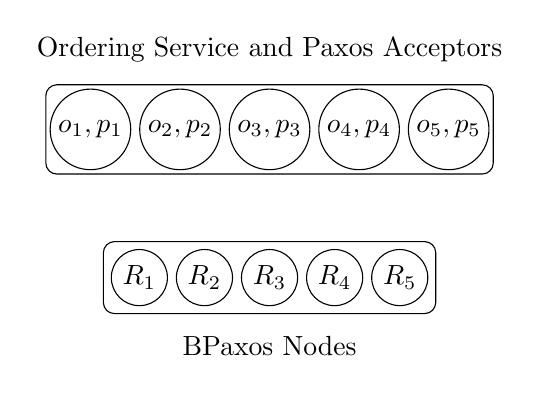
\begin{tikzpicture}
    \tikzstyle{machine}=[draw, circle, inner sep=2pt]

    % Ordering Service / Paxos Acceptors
    \node[machine] (o1) at (0, 2) {$o_1, p_1$};
    \node[machine, right=0.1cm of o1] (o2) {$o_2, p_2$};
    \node[machine, right=0.1cm of o2] (o3) {$o_3, p_3$};
    \node[machine, right=0.1cm of o3] (o4) {$o_4, p_4$};
    \node[machine, right=0.1cm of o4] (o5) {$o_5, p_5$};
    \node (os) at ($(o3.north) + (0, 0.5)$) {Ordering Service and Paxos Acceptors};
    \draw[rounded corners]
      ($(o1.south west) + (-0.2, -0.2)$) rectangle
      ($(o5.north east) + (0.2, 0.2)$);

    % BPaxos Nodes
    \node[machine, below=1cm of o3] (b3) {$R_3$};
    \node[machine, left=0.1cm of b3] (b2) {$R_2$};
    \node[machine, left=0.1cm of b2] (b1) {$R_1$};
    \node[machine, right=0.1cm of b3] (b4) {$R_4$};
    \node[machine, right=0.1cm of b4] (b5) {$R_5$};
    \draw[rounded corners]
      ($(b1.south west) + (-0.2, -0.2)$) rectangle
      ($(b5.north east) + (0.2, 0.2)$);
      \node (bpaxos) at ($(b3.south) + (0, -0.5)$) {BPaxos Nodes};
  \end{tikzpicture}

  \caption{Colocated BPaxos}\figlabel{ColocatedBPaxos}
\end{figure}
}

Second, we implement our consensus service using Fast Paxos instead of regular
Paxos. We let ballot $0$ be a fast ballot and every other ballot be a classic
ballot. As before, every BPaxos instance $R$ runs phase 1 of Fast Paxos for
every instance $R.i$. In the normal case, $R$ finishes executing phase 1 and
sends phase 2a ``any'' messages to the Fast Paxos acceptors. At this point, the
acceptors are free to vote for the first proposal that they hear from anyone
(not just from $R$).

As before, when a BPaxos node $R$ receives a command $a$ from a client, it
sends the command to the ordering service nodes in some instance $R.i$. Upon
receiving $a$, an ordering service node $o_j$ computes its reply $(R.i, a,
\deps{a}_j)$. Unlike with BPaxos, $o_j$ does not return the reply $(R.i, a,
\deps{a}_j)$ directly to $R$. Instead, it proposes the value $(a, \deps{a}_j)$
in instance $R.i$ to $p_j$ (the colocated Fast Paxos acceptor). As we just
described, $p_j$ votes for the first proposal that it hears from anyone, so
$p_j$ votes for the value $(a, \deps{a}_j)$ in instance $R.i$ and relays its
phase 2b vote back to $R$.

If $R$ receives a superquorum (i.e.\ $f + \floor{\frac{f+1}{2}} + 1$) of phase
2b votes for the same value $(a, \deps{a}_{j_1}) = \cdots = (a,
\deps{a}_{j_{m}})$ in instance $R.i$, then Fast Paxos (and hence BPaxos)
considers the value chosen. Thus, in the best case, BPaxos can commit a value
in one round trip to a superquorum (just like EPaxos).

If $R$ does \emph{not} receive a superquorum of phase 2b votes for the same
value, then it is unsure whether or not a value was chosen and begins
\defword{recovery} for instance $R.i$. We'll explain recovery in one moment. At
any point in time, any other BPaxos node $Q$ may also begin recovery for
instance $R.i$. In practice, a BPaxos node will only begin recovery if it
believes $R$ has failed, but any node may attempt to recover any instance at
any time.

In this incorrect BPaxos variant, the recovery of instance $R.i$ by node $Q$ is
simply the process of $Q$ attempting to get a value chosen in $R.i$ with a
higher ballot. In particular, $Q$ runs the Fast Paxos variant described in
\secref{FastPaxos}. If $Q$ reaches Case 3 of Fast Paxos, it proposes $(\noop,
\emptyset)$.

\paragraph{Incorrectness}
Now, we explore why this variant of BPaxos is incorrect. Assume we are running
this BPaxos variant with $f = 2$, and imagine EPaxos node $Q$ is attempting to
recovery instance $R.i$. $Q$ begins Fast Paxos with ballot 1 and sends phase 1a
messages to some majority of consensus nodes. $Q$ receives the following phase
1b messages from a majority of acceptors:
\begin{itemize}
  \item
    $p_3$ voted for $(a, \set{I_b})$ in round $0$.
  \item
    $p_4$ voted for $(a, \set{I_b})$ in round $0$.
  \item
    $p_4$ voted for $(a, \set{I_c})$ in round $0$.
\end{itemize}
where $I_b$ is an instance with command $b$ and $I_c$ is an instance with
command $c$.
%
$Q$ then begins phase 2 of Fast Paxos. $p_3$ and $p_4$ voted for the value $(a,
\set{b})$ in round $0$. $p_1$ and $p_2$ maybe also voted for $(a, \set{I_b})$
in round $0$, which means that $(a, \set{I_b})$ may have been chosen in round
$0$. Thus, $Q$ executes Case 2 and proposes that the value $(a, \set{I_b})$ be
chosen.

This is incorrect! It's possible that $p_1$ and $p_2$ did \emph{not} vote for
$(a, \set{I_b})$ in round $0$. For example, they could have voted for $(a,
\set{I_c})$. In this case, $\set{I_b}$, the dependencies proposed by $Q$, are
not the union of responses from a majority of ordering service nodes. Because
of this, this incorrect BPaxos variant does not maintain
\invref{ConflictingGadgets}.

More concretely, we can construct the following execution of this incorrect
BPaxos variant in which two conflicting commands are both chosen and neither
depends on the other. $R$ receives command $a$ and $Q$ receives a conflicting
command $b$.  $o_1$ and $o_2$ receive $a$ and propose $(a, \emptyset)$ in
instance $R.i$ to acceptors $p_1$ and $p_2$. Similar, $o_4$ and $o_5$ receive
$b$ and propose $(b, \emptyset)$ in instance $Q.j$ to acceptors $p_4$ and
$p_5$. Then, $R$ and $Q$ crash and all other messages are dropped. Another
BPaxos node $S$ attempts to recover $R.i$. In phase 1 of Fast Paxos, it hears
from $p_1$, $p_2$, and $p_3$, and then gets the value $(a, \emptyset)$ chosen.
Then, another node $T$ recovers $Q.j$. In phase 1 of Fast Paxos, it hears from
$p_3$, $p_4$, and $p_5$ and then gets the value $(b, \emptyset)$ chosen. $S$
executes $a$ and $T$ executes $b$.

Taking a step back, we see that this BPaxos variant is incorrect because it
fails to maintain \invref{ConflictingGadgets}. It fails to maintain this
invariant because of a mismatch between the invariants that BPaxos wants to
maintain and the invariants that Fast Paxos provides. BPaxos wants to get
values of the form $(a, \deps{a})$ chosen, but only if $\deps{a}$ is the union
of responses from a majority of ordering service nodes. This is required to
ensure that conflicting commands will depend on one another. However Fast
Paxos wants to get \emph{any} value chosen. Fast Paxos has no understanding of
the ordering service nodes, or any notion that some specific values should not
be chosen. Fast Paxos tries to get any proposed value chosen. In our example
above, when node $S$ received 2 votes for $(a, \emptyset)$ in round 0, Fast
Paxos determined that this value may have been chosen in round 0, so it happily
proposes it. Fast Paxos doesn't understand the additional requirement that
BPaxos requires: that $(a, \emptyset)$ cannot be chosen unless a majority of
ordering service nodes determined that $a$'s dependencies should be the empty
set.

Here's another way to interpret the incorrectness of this BPaxos variant. When
a node $Q$ is recovering an instance $R.i$ and wants to propose a value $v =
(a, \deps{a})$, it has to perform the logic illustrated in
\figref{BPaxosLogic}.
%
If it's possible that a value $v$ was previously chosen, then to avoid choosing
two different values, we have no choice but to propose $v$.
%
Similarly, if $v$ is a union of responses from a majority of ordering service
nodes, then we're free to propose it, but if $v$ is not the union of responses
from a majority of ordering service nodes, then we can't propose it.
%
If a recovering node $Q$ has a value $v$ that may have been chosen \emph{and}
is maybe not a union of responses from a majority of ordering service nodes,
then $Q$ is stuck. It simultaneously has to propose $v$ and cannot propose $v$.
This is exactly the situation in which our BPaxos variant is incorrect. When
faced with such a value $v$, it erroneously proposes $v$.

\begin{figure}[h]
  \centering
  \begin{tabular}{rccc}
    %
    &
    &
    \multicolumn{2}{p{3in}}{%
      Is $v$ a union of responses from a majority of ordering service nodes?%
    } \\
    %
    &
    &
    yes &
    maybe not \\\cline{3-4}
    %
    \multirow{2}{1.8in}{Was $v$ previously chosen?} &
    maybe &
    \multicolumn{1}{|c|}{Propose it} &
    \multicolumn{1}{|c|}{We're stuck!} \\\cline{3-4}
    %
    &
    definitely not &
    \multicolumn{1}{|c|}{Propose it, or propose noop} &
    \multicolumn{1}{|c|}{Propose noop} \\\cline{3-4}
  \end{tabular}
  \caption{The logic that any BPaxos variant should follow}%
  \figlabel{BPaxosLogic}
\end{figure}

Thus, in order for a BPaxos variant to be correct, it has to eliminate the
possibility that a value $v$ may have been chosen and simultaneously may not be
a union of responses from a majority of ordering service nodes. In the next
couple of sections, we'll introduce a couple of BPaxos variants. We'll see that
each variant uses different mechanisms to ensure that this situation is
impossible.

\section{Unanimous Bipartisan Paxos}\seclabel{UnanimousBPaxos}
\paragraph{Overview}
Take the incorrect BPaxos variant from the previous section and increase the
Fast Paxos superquorum sizes from $f + \floor{\frac{f+1}{2}} + 1$ to $2f + 1$.
That is, choosing a value in a fast round requires a unanimous vote. We call
this variant \defword{Unanimous BPaxos}. This variant, like the incorrect
variant from the previous section, can commit a command in one round trip (in
the best case), but unlike the previous variant, this variant is correct.

\paragraph{Correctness}
Unanimous BPaxos maintains \invref{GadgetsChosen} trivially. To prove Unanimous
BPaxos maintains \invref{ConflictingGadgets}, we prove the claim $P(i)$ that
says if a Fast Paxos acceptor votes for value $(a, \deps{a})$ in round $i$,
then either
\begin{itemize}
  \item
    $i = 0$, or
  \item
    $\deps{a}$ is the union of responses from a majority of ordering service
    nodes, or
  \item
    $(a, \deps{a}) = (\noop, \emptyset)$.
\end{itemize}
We prove this by induction. $P(0)$ is trivial; the first disjunct is satisfied.
For the general case, we perform a case analysis on the proposer's logic. Call
this proposer $Q$.
\begin{itemize}
  \item (Case 1)
    $V = \set{(a, \deps{a})}$ and $k \neq 0$. $P(i)$ holds directly from
    $P(k)$.

  \item (Case 2)
    If $k \neq 0$, then $P(i)$ holds directly from $P(k)$. Otherwise, $k = 0$.
    It's only possible that value $(a, \deps{a})$ was chosen in round $0$ if
    some proposer received phase 1b messages from every acceptor such that the
    acceptors unanimously voted for $(a, \deps{a})$.

    In this case, the quorum of phase 1b messages that $Q$ received is also a
    unanimous vote for $(a, \deps{a})$.  Thus, $\deps{a}$ is the union of
    responses from a majority of ordering service nodes (the majority that $Q$
    contacted), so the second disjunct of $P(i)$ holds.

  \item (Case 3)
    In this case, a proposer always chooses to propose a $\noop$, so $P(i)$
    holds trivially.
\end{itemize}

It follows that Unanimous BPaxos maintains \invref{ConflictingGadgets} and is
therefore correct. But, let's not miss the forest through the proof. Let's take
a step back and think about why increasing the superquorum size from $f +
\floor{\frac{f+1}{2}} + 1$ to $2f+1$ turns our incorrect BPaxos variant into a
correct one. Referring to \figref{BPaxosLogic}, we see that the top right
corner is now impossible. If a Unanimous BPaxos node concludes that a value
$(a, \deps{a})$ was maybe previously chosen, then it knows for sure that
$\deps{a}$ was a union of responses from a majority of ordering service nodes.

\section{Fast Bipartisan Paxos}
In this section, we present \defword{Fast Bipartisan Paxos}. Fast BPaxos can
commit commands in one round trip like Unanimous BPaxos, but Fast BPaxos only
requires a superquorum size of $f + \floor{\frac{f}{2}} + 1$.

\paragraph{Ordering Service}
Fast BPaxos' ordering service is implemented as a slight tweak to BPaxos'
ordering service. The tweak enables ordering service nodes to remember their
responses and resend them at a later time. We'll explain the small tweak
momentarily, and later it will become clear why we need this tweak, but first,
it's important to note that though the implementations of Fast BPaxos' ordering
service and BPaxos' ordering service are different, their guarantees are the
same. Namely, they both maintain \invref{OrderingService}.

\newcommand{\out}{\text{out}}
A Fast BPaxos ordering service node $o_i$ maintains a directed acyclic graph
$G_i$. Every vertex of the graph is labelled with a Fast BPaxos instance and
contains a state machine command. When $o_i$ receives a command $a$ for
instance $I_a$ from a Fast BPaxos node, it performs the following actions:
\begin{enumerate}
  \item
    Let $\out(I_a)$ be the set of outbound edges emanating from the vertex
    labelled $I_a$. If there is already a vertex in $G_i$ labelled $I_a$,
    then $o_i$ returns $(I_a, a, \out(I_a))$ and does nothing else. As with
    BPaxos' ordering service, Fast BPaxos' ordering service assumes that at
    most one command can be sent in any given instance. So, the command stored
    in vertex $I_a$ must be $a$.
  \item
    If there does not exist a vertex labelled $I_a$ in $G_i$, then $o_i$
    inserts a vertex into $G_i$ with label $I_a$ and with command $a$. An edge
    is added from instance $I_a$ to instance $I_b$ for every other instance
    $I_b$ in the graph that contains a command $b$ that conflicts with $a$.
    $o_i$ then returns the tuple $(I_a, a, \out(I_a))$.
\end{enumerate}

An example of such a graph is given in
\figref{FastPaxosOrderingServiceCartoonBefore}. The same graph is shown
\figref{FastPaxosOrderingServiceCartoonAfter}, except that the command $e$ has
arrived in instance $Q.2$ and conflicts with commands $c$ and $d$.
%
There are a couple of things worth noting about an ordering service node $o_i$
and the corresponding graph $G_i$.
\begin{itemize}
  \item
    $G_i$ is always acyclic.
  \item
    One a gadget $(I_a, a, \out(I_a))$ is inserted into $G_i$, the gadget is
    never modified.
  \item
    The edges in $G_i$ reflect the order in which conflicting commands were
    received by $o_i$. If there is an edge from instance $I_a$ to instance
    $I_b$, then $o_i$ must have received command $b$ in $I_b$ before receiving
    command $a$ in $I_a$.
  \item
    EPaxos, BPaxos, Unanimous BPaxos, and Fast BPaxos all construct a directed
    cyclic graph of commands that are then executed in reverse topological
    order by strongly component. This graph is not the same graph as $G_i$.
    $G_i$ is a completely separate graph that serves a completely different
    purpose.
\end{itemize}

\begin{figure}[h]
  \centering

  \begin{subfigure}[b]{0.35\textwidth}
    \begin{tikzpicture}[scale=2.5]
      \node[square] (a) at (0, 1) {$a$};
      \node[square] (b) at (0, 0) {$b$};
      \node[square] (c) at (1, 1) {$c$};
      \node[square] (d) at (1, 0) {$d$};
      \draw[ultra thick, -latex] (c) to (a);
      \draw[ultra thick, -latex] (c) to (b);
      \draw[ultra thick, -latex] (d) to (b);
      \foreach \label/\i in {a/$R.1$, b/$R.2$, c/$Q.1$, d/$S.1$} {%
        \node[above=0in of \label] {\i};
      }
    \end{tikzpicture}
    \caption{}\figlabel{FastPaxosOrderingServiceCartoonBefore}
  \end{subfigure}
  %
  \begin{subfigure}[b]{0.35\textwidth}
    \begin{tikzpicture}[scale=2.5]
      \node[square] (a) at (0, 1) {$a$};
      \node[square] (b) at (0, 0) {$b$};
      \node[square] (c) at (1, 1) {$c$};
      \node[square] (d) at (1, 0) {$d$};
      \node[square] (e) at (2, 0.5) {$e$};
      \draw[ultra thick, -latex] (c) to (a);
      \draw[ultra thick, -latex] (c) to (b);
      \draw[ultra thick, -latex] (d) to (b);
      \draw[ultra thick, -latex] (e) to (c);
      \draw[ultra thick, -latex] (e) to (d);
      \foreach \label/\i in {a/$R.1$, b/$R.2$, c/$Q.1$, d/$S.1$, e/$Q.2$} {%
        \node[above=0in of \label] {\i};
      }
    \end{tikzpicture}
    \caption{}\figlabel{FastPaxosOrderingServiceCartoonAfter}
  \end{subfigure}

  \caption{%
    (left) A directed acyclic graph stored at a Fast BPaxos ordering service
    node. (right) The same graph after the command $e$ arrives in instance
    $Q.2$.
  }\figlabel{FastPaxosOrderingServiceCartoon}
\end{figure}

Taking a step back, we see that Fast BPaxos' ordering service is more or less
the same as BPaxos's ordering service. The only difference is that a Fast
BPaxos node can send a command $a$ in instance $I_a$ to an ordering service
multiple times. The first time an ordering service node receives $(I_a, a)$, it
behaves identically to BPaxos' ordering service. Every subsequent time it
receives $(I_a, a)$, it sends back its original reply.

\paragraph{Consensus Service}
Like Unanimous BPaxos, Fast BPaxos implements the consensus service with Fast
Paxos. Like Unanimous BPaxos, every Fast BPaxos instance has a corresponding
Fast Paxos instance. Like Unanimous BPaxos, round 0 of every instance is a
fast ballot and every other round is a classic ballot.
%
The one difference is that Fast BPaxos uses superquorums of size $f +
\floor{\frac{f}{2}} + 1$, the same as regular Fast Paxos.

\paragraph{Fast BPaxos Nodes}
In the normal case, Fast BPaxos nodes behave exactly like Unanimous BPaxos
nodes. Upon receiving a command $a$ from a client, a Fast BPaxos node $R$
chooses some previously unused instance $R.i$ for the command. It then sends
$(R.i, a)$ to the ordering service nodes.
%
When an ordering service node $o_j$ receives $(R.i, a)$, it proposes it's reply
$(R.i, a, \deps{a}_j)$ to $p_j$, the colocated Paxos acceptor. $p_j$ then sends
its vote back to $R$.
%
If $R$ receives a superquorum of matching votes $(R.i, a, \deps{a})$, then the
gadget is considered chosen. If it does not receive a superquorum of matching
votes, it enters recovery.

Recovery is where Unanimous BPaxos and Fast BPaxos differ. To understand Fast
BPaxos' recovery, we first have to understand one of the key invariants that it
maintains. Recall that both BPaxos and Unanimous BPaxos maintain the invariant
that a BPaxos node can only propose a value $(a, \deps{a})$ in instance $I_a$
if either (a) $(I_a, a, \deps{a})$ was a response from the ordering service or
(b) $a = \noop$ and $\deps{a} = \emptyset$. Doing so,
\invref{ConflictingGadgets} followed trivially from \invref{OrderingService}.

Fast BPaxos will maintain an invariant that is slightly weaker (and hence
easier to maintain) but still strong enough to imply
\invref{ConflictingGadgets}. The motivation for the weaker invariant is as
follows. Imagine a Fast BPaxos node $R$ sends command $a$ to the ordering
service in instance $I_a$, and the ordering service responds with $(I_a, a,
\deps{a})$. Let $I_b \in \deps{a}$ be one of $a$'s dependencies. Assume that
that $R$ knows that $I_b$ has been committed with command $b$ and dependencies
$\deps{b}$. Further assume that $I_a \in \deps{b}$. That is, there is an edge
from $I_b$ to $I_a$. In this case, there is no need for $R$ to include $I_b$ in
the dependencies of $I_a$! \invref{ConflictingGadgets} asserts that if two
committed commands conflict, one has an edge to the other (or both). If $I_b$
has already committed with an edge to $I_a$, there is no need to propose an
edge from $I_a$ back to $I_b$.
%
Similarly, if $I_b$ has been committed with a $\noop$, then there is no need to
propose an edge from $I_a$ to $I_b$ at all because $a$ and $\noop$ do not
conflict.

\newcommand{\pruned}{\text{pruned}}
Let $(I_a, a, \deps{a})$ be a response from the ordering service. Let $P$ be
the set of instances $I_c$ in $\deps{a}$ such that $I_c$ has been committed
with $I_a$ in its dependencies or $c$ is a $\noop$. Then, we call
$\pruned(\deps{a}) = \deps{a} - P$ the \defword{pruned dependencies} of $I_a$
(or $a$). Fast BPaxos maintains the following invariant:

\begin{boxedinvariant}\invlabel{PrunedDependencies}
  A Fast BPaxos node will only propose a value $(a, \deps{a})$ in instance
  $I_a$ if $(I_a, a, \deps{a})$ is a pruned response from the ordering service
  or if $a = \noop$ and $\deps{a} = \emptyset$.
\end{boxedinvariant}

To recover a Fast BPaxos instance $I_a$, a Fast BPaxos node $Q$ runs through
the normal Fast Paxos protocol in an attempt to get a value chosen in instance
$I_a$. $Q$ executes Case 1 unchanged. If $Q$ enters Case 3 of Fast Paxos, it
proposes $(\noop, \emptyset)$ in $I_a$. If $Q$ enters Case 2 with some value
$v$, then it has some hard work to do.

Case 2 is the scenario outlined in \figref{BPaxosLogic} where $(a, \deps{a})$
may have been previously chosen, and $\deps{a}$ may not be a pruned response
from the ordering service. $Q$ is stuck. To get unstuck, $Q$ has to do one of
two things. It either has to determine that $\deps{a}$ is a pruned response
from the ordering service, or it has to determine that $(a, \deps{a})$ was
definitely not previously chosen.

\tikzstyle{smallsquare}=[%
  draw,
  line width=1pt,
  minimum height=0.4in,
  minimum width=0.3in,
  text width=0.3in,
  align=center
]
\begin{figure}[ht]
  \centering
  \begin{tikzpicture}[xscale=2.5, yscale=2]
    \node[smallsquare] (a) at (1, 1) {$a$};
    \node[smallsquare] (dep1) at (0.5, 0) {$b_1$};
    \node[smallsquare] (dep2) at (1, 0) {$b_2$};
    \node[smallsquare] (dep3) at (1.5, 0) {$b_3$};
    \node[smallsquare] (c) at (2, 1) {$c$};

    \node[above=0in of a] {$I_a$};
    \node[below=0in of dep1] {$I_{b_1}$};
    \node[below=0in of dep2] {$I_{b_2}$};
    \node[below=0in of dep3] {$I_{b_3}$};
    \node[above=0in of c] {$I_c$};

    \draw[ultra thick, -latex] (a) to (dep1);
    \draw[ultra thick, -latex] (a) to (dep2);
    \draw[ultra thick, -latex] (a) to (dep3);
    \draw[ultra thick, -latex] (a) to (c);

    \node[%
      draw=red,
      line width=1pt,
      rounded rectangle,
      minimum width=2in,
      minimum height=1in,
      label={270:$\deps{a}$}
    ] () at (dep2) {};
  \end{tikzpicture}
  \caption{Fast BPaxos recovery comic}\figlabel{FastBPaxosNotUnion}
\end{figure}

First, $Q$ sends $(I_a, a)$ to a quorum $\mathcal{Q}$ of $f + 1$ ordering
service nodes%
\footnote{%
  Note that $Q$ has already contacted a quorum of $f + 1$ Fast Paxos nodes as
  part of Fast Paxos. When $Q$ contacts Fast Paxos acceptor $p_j$, it can
  simultaneously send $(I_a, a)$ to the colocated ordering service node $o_j$.
}
and receives responses $(I_a, a, \deps{a}_{j_1}), \ldots, (I_a, a,
\deps{a}_{j_{f+1}})$. If $\deps{a} = \pruned(\cup_j \deps{a}_j)$, then we're
unstuck. $\deps{a}$ is a pruned response from the ordering service, so $Q$ can
propose $(a, \deps{a})$.
%
Otherwise, there is some $(I_a, a, \deps{a}_j)$ where $\deps{a}_j$ includes an
unpruned instance $I_c$ with command $c$ that is not in $\deps{a}$. This is
illustrated in \figref{FastBPaxosNotUnion}. $Q$ proceeds as follows.
\begin{itemize}
  \item
    If $Q$ knows that $(I_c, c, \deps{c})$ has been chosen:
    \begin{itemize}
      \item
        We know that $c \neq \noop$ and that $I_a \notin \deps{c}$ because
        $I_c$ was not pruned.

      \item
        By \invref{PrunedDependencies}, $\deps{c}$ must be a pruned response
        from the ordering service. $I_a$ has not yet been commited, so $I_a$
        cannot have been pruned from $\deps{c}$. Thus, there is a majority of
        ordering service nodes that saw $c$ before $a$.
        %
        \todo{mwhittaker}{%
          I think this is actually a little subtle. Maybe some other node has
          gotten $I_a$ committed in the meantime with $I_c$ in its
          dependencies. Maybe, but then this Fast Paxos round will fail, so it
          should be okay. We'll need to formalize pruning more.%
        }

      \item
        Thus, it is impossible that $(a, \deps{a})$ was chosen by a superquorum
        in round $k$ because $I_c \notin \deps{a}$, so there must have been a
        superquorum of nodes that saw $a$ before $c$.
        %
        \todo{mwhittaker}{%
          Elaborate a bit that we can only hit Case 2 when $k = 0$ since it is
          the only fast ballot.%
        }

      \item
        Thus, we are free to propose $(\noop, \emptyset)$.
    \end{itemize}
  \item
    Otherwise:
    \begin{itemize}
      \item
        $Q$ starts recovery for $I_c$ to have $I_c$ chosen. $Q$ makes sure to
        contact the same quorum $\mathcal{Q}$. If after a timeout, the same
        quorum cannot be reached, then it's possible some node in the quorum
        has failed. If so, $Q$ will start recovery over for every instance with
        some new quorum. One quorum is guaranteed to exist since at most $f$
        nodes can fail.
        %
        \todo{mwhittaker}{%
          This is theoretically nice, but implementation-wise a nightmare. I
          think we can get around this and allow disjoint quorums, but then the
          algorithm will have to do something smarter to avoid deadlock.
          %
          We may be able to have an ordering service node return not only the
          deps of a command, but all of its deps, and so on transitively. If we
          don't want to enforce the same quorum, there probably has to be some
          logic along the lines of figuring out when some $M$ must lie in the
          superquorum of some other command which means there has to be an
          abort somewhere.%
        }

      \item
        After $I_c$ has been chosen, $Q$ re-prunes $\deps{a}$ and repeats this
        loop.

      \item
        Eventually, every $I_c$ will either be (1) chosen as a $\noop$ in which
        case it is pruned, (2) chosen with an edge to $I_a$ in which case it is
        pruned, or (3) chosen without an edge to $I_a$ in which case we propose
        $(\noop, \emptyset)$.
    \end{itemize}
\end{itemize}

This is the entirety of the Fast BPaxos algorithm, but there is one small
detail remaning. A node $Q$ recovering $I_a$ may block until it recovers $I_c$.
Can $I_c$ block recovering $I_a$? Or more generally, can a node deadlock itself
during recovery? The answer is no. Let's prove it.

Assume for contradiction there existed a sequence
$
  (I_{a_1}, a_1, \deps{a_1}),
  \ldots
  (I_{a_r}, a_r, \deps{a_r})
$
of gadgets such that the recovery of $a_i$ is blocked on the recovery of
$a_{i+1}$ (with wraparound). We know $a_{i+1} \notin \deps{a_i}$ for every $i$.
%
Some majority of $\mathcal{Q}$, say $M_1$, of nodes unanimously voted for
$\deps{a_1}$ in some round $k$. Every node in $M_1$ saw $a_1$ before $a_2$.
Otherwise, $I_{a_2}$ would be in $\deps{a_1}$.
%
Similarly, some majority $\mathcal{Q}$, say $M_2$, of nodes unanimously voted
for $\deps{a_2}$ in some round $k$. Every node in $M_2$ saw $a_2$ before $a_3$.
Otherwise, $I_{a_3}$ would be in $\deps{a_2}$.
%
Consider some node $o_i \in M_1 \cap M_2$ (which is guaranteed to be
non-empty). Then, $o_i$ saw $a_1$ before $a_2$ before $a_3$. Moreover, every
node in $M_2$ computed the same dependencies, so in fact, every node in $M_2$
saw $a_1$ before $a_2$ before $a_3$. Repeating this argument for every $i$,
we'll eventually find that every node has seen $a_1$ before $a_1$. This is a
contradiction.

\paragraph{Correctness}
\todo{mwhittaker}{Prove correctness more formally.}

\bibliographystyle{plain}
\bibliography{references}

\begin{appendices}

\section{An Aside on Fast Paxos}\seclabel{FastPaxos}
Before we move on, we summarize the relevant bits of Fast
Paxos~\cite{lamport2006fast} that are critical to our remaining BPaxos
variants. In Fast Paxos, after a proposer receives phase 1b messages from a
quorum of acceptors, it performs the following logic to select a value to
propose:
\begin{itemize}
  \item
    Let $k$ be the largest vote round in the quorum of phase 1b messages.
    Let $V$ be the corresponding set of vote values for round $k$.
  \item
    (Case 1) If $V = \set{v}$, then propose $v$.
  \item
    (Case 2) If $V$ contains a value $v$ that may have been chosen in round
    $k$, propose $v$. Note that quorum sizes are selected in such a way that at
    most one such $v$ can exist.
  \item
    (Case 3) Otherwise, propose anything.
\end{itemize}

Proving the correctness of Fast Paxos involves proving the statement $P(i)$
that says that if an acceptor votes for a value $v$ in round $i$, then no
other value besides $v$ has been or will be chosen in any round $j$ less than
$i$. We prove this claim by induction. $P(0)$ is trivial because there are no
rounds less than $0$. For the general case, we perform a case analysis on $j$.
First, assume $k \neq -1$.
\begin{itemize}
  \item
    If $k < j < i$, then no value has been or will be chosen in round $j$
    because a phase 1 quorum of acceptors had not voted in any round larger
    than $k$ and promised not to vote in any round less than $i$.

  \item
    If $k = j$, then we perform a case analysis on the proposer's logic.
    \begin{itemize}
      \item
        (Case 1) If $V = \set{v}$, then a quorum of acceptors have either voted
        for $v$ in round $k$ or promised not to vote in round $k$. Thus, no
        other value besides $v$ can be chosen in round $k$.
      \item
        (Case 2) If $V$ contains a value that may have been chosen in round
        $k$, we propose it. Quorum sizes are set up such that no other value
        could have been chosen in round $k$.
      \item
        (Case 3) No value could have been chosen in round $k$.
    \end{itemize}

  \item
    If $j < k$, we again perform a case analysis on the proposer's logic.
    \begin{itemize}
      \item
        (Case 1) By $P(k)$, no value other than $v$ has been or will be chosen
        in round $j$.
      \item
        (Case 2) Let $v_1, v_2 \in V$. By $P(v_1), P(v_2)$, no value has been
        or will be chosen in round $j$.
      \item
        (Case 3) Same as Case 2.
    \end{itemize}
\end{itemize}
If $k = -1$, then we know that no value has been or will be chosen in any round
less than $i$ by the same line of reasoning as above, so we're free to propose
anything.

Note that we can make the following small tweak to Fast Paxos without
compromising its correctness. We can change Case 1 of the proposer's logic from
``If $V = \set{v}$, then propose $v$'' to ``If $V = \set{v}$ and $k \neq 0$,
then propose $v$''. That is, a proposer will only perform Case 1 if $k \neq 0$.

\section{Reducing $\noop$s}
TODO: Mention how we can avoid sending too many noops by having BPaxos nodes
send a union of votes instead of noops.

TODO: Explain that Unanimous BPaxos and Fast BPaxos can be "fast" in the sense
of fast paxos. Clients can initiate the protocol. They don't have to send to a
command leader first. The one wrinkle is that a client will have to randomly
pick a leader for the instance, say $R$, and send the command in some fresh
instance owned by $R$. These fresh instances have to be default initialized in
the any state, but this doesn't affect the correctness of anything.

\end{appendices}
\end{document}
